\documentclass[english,11pt,table,handout]{beamer}

% Copyright 2007 by Till Tantau
%
% This file may be distributed and/or modified
%
% 1. under the LaTeX Project Public License and/or
% 2. under the GNU Public License.
%
% See the file doc/licenses/LICENSE for more details.


% Common packages
\usepackage[utf8x]{inputenc}
\usepackage[vietnam,english]{babel}
\usepackage[utf8]{vietnam}
%\usepackage{times}
\usefonttheme[onlymath]{serif}
\usecolortheme{default}
\usepackage{booktabs}
\usepackage{mathpartir}
\usepackage{listings}
\usepackage{listingsutf8}

\usepackage{pbox}
\mprset{flushleft}
\mode<article>
{
  \usepackage{times}
  \usepackage{mathptmx}
  \usepackage[left=1.5cm,right=6cm,top=1.5cm,bottom=3cm]{geometry}
}

\usepackage{hyperref}
\usepackage{tikz}
\usetikzlibrary{arrows,backgrounds}
%\tikzstyle{mnode}=[circle, draw, fill=black, inner sep=0pt, minimum width=4pt]
\usepackage{colortbl}
%\usepackage{yfonts}
\usepackage{translator} % comment this, if not available


% Common settings for all lectures in this course

\def\lecturename{Image Processing and Computer Vision}

\title{\insertlecture}

\author{\textbf{LE Thanh Sach}}

\institute
{
  \textit{Faculty of Computer Science and Engineering}\\
  \textit{Ho Chi Minh University of Technology, VNU-HCM}
}

\subject{Lecturer \lecturename}

% Beamer version theme settings

\useoutertheme[height=0pt,width=2cm,right]{sidebar}
\usecolortheme{rose,sidebartab}
\useinnertheme{circles}
\usefonttheme[only large]{structurebold}

\setbeamercolor{sidebar right}{bg=black!15}
\setbeamercolor{structure}{fg=blue}
\setbeamercolor{author}{parent=structure}

\setbeamerfont{title}{series=\normalfont,size=\LARGE}
\setbeamerfont{title in sidebar}{series=\bfseries}
\setbeamerfont{author in sidebar}{series=\bfseries}
\setbeamerfont*{item}{series=}
\setbeamerfont{frametitle}{size=}
\setbeamerfont{block title}{size=\small}
\setbeamerfont{subtitle}{size=\normalsize,series=\normalfont}

\setbeamertemplate{navigation symbols}{}
\setbeamertemplate{bibliography item}[book]
\setbeamertemplate{sidebar right}
{
  {\usebeamerfont{title in sidebar}%
    \vskip1.5em%
    \hskip3pt%
    \usebeamercolor[fg]{title in sidebar}%
    \insertshorttitle[width=2cm,center,respectlinebreaks]\par%
    \vskip1.25em%
  }%
  {%
    \hskip3pt%
    \usebeamercolor[fg]{author in sidebar}%
    \usebeamerfont{author in sidebar}%
    \insertshortauthor[width=2cm,center,respectlinebreaks]\par%
    \vskip1.25em%
  }%
  \hbox to2cm{\hss\insertlogo\hss}
  \vskip1.25em%
  \insertverticalnavigation{2cm}%
  \vfill
  \hbox to 2cm{\hfill\usebeamerfont{subsection in
      sidebar}\strut\usebeamercolor[fg]{subsection in
      sidebar}\insertshortlecture.\insertframenumber\hskip5pt}%
  \vskip3pt%
}%

\setbeamertemplate{title page}
{
  \vbox{}
  \vskip1em
  {\huge Chapter \insertshortlecture\par}
  {\usebeamercolor[fg]{title}\usebeamerfont{title}\inserttitle\par}%
  \ifx\insertsubtitle\@empty%
  \else%
    \vskip0.25em%
    {\usebeamerfont{subtitle}\usebeamercolor[fg]{subtitle}\insertsubtitle\par}%
  \fi%     
  \vskip1em\par
  \emph{\lecturename}\ 
  %on \insertdate\par
  \vskip3em\par

  \leftskip=0pt plus1fill\insertauthor\par
  \insertinstitute\vskip1em
}

\logo{
\includegraphics[width=1.5cm]{hcmut.png}}



% Article version layout settings

\mode<article>

\makeatletter
\def\@listI{\leftmargin\leftmargini
  \parsep 0pt
  \topsep 5\p@   \@plus3\p@ \@minus5\p@
  \itemsep0pt}
\let\@listi=\@listI


\setbeamertemplate{frametitle}{\paragraph*{\insertframetitle\
    \ \small\insertframesubtitle}\ \par
}
\setbeamertemplate{frame end}{%
  \marginpar{\scriptsize\hbox to 1cm{\sffamily%
      \hfill\strut\insertshortlecture.\insertframenumber}\hrule height .2pt}}
\setlength{\marginparwidth}{1cm}
\setlength{\marginparsep}{4.5cm}

\def\@maketitle{\makechapter}

\def\makechapter{
  \newpage
  \null
  \vskip 2em%
  {%
    \parindent=0pt
    \raggedright
    \sffamily
    \vskip8pt
    {\fontsize{36pt}{36pt}\selectfont Chapter \insertshortlecture \par\vskip2pt}
    {\fontsize{24pt}{28pt}\selectfont \color{blue!50!black} \insertlecture\par\vskip4pt}
    {\Large\selectfont \color{blue!50!black} \insertsubtitle\par}
    \vskip10pt

    \normalsize\selectfont Print version of
    Lecturer \emph{\lecturename} of \@date\par\vskip1.5em
    %\hfill Le Thanh Sach and Luong The Nhan, Faculty of CSE, HCMC University of Technology
  }
  \par
  \vskip 1.5em%
}

\let\origstartsection=\@startsection
\def\@startsection#1#2#3#4#5#6{%
  \origstartsection{#1}{#2}{#3}{#4}{#5}{#6\normalfont\sffamily\color{blue!50!black}\selectfont}}

\makeatother

\mode
<all>




% Typesetting Listings

\usepackage{listings}
\lstset{language=Java}

\alt<presentation>
{\lstset{%
  basicstyle=\footnotesize\ttfamily,
  commentstyle=\slshape\color{green!50!black},
  keywordstyle=\bfseries\color{blue!50!black},
  identifierstyle=\color{blue},
  stringstyle=\color{orange},
  escapechar=\#,
  emphstyle=\color{red}}
}
{
  \lstset{%
    basicstyle=\ttfamily,
    keywordstyle=\bfseries,
    commentstyle=\itshape,
    escapechar=\#,
    emphstyle=\bfseries\color{red}
  }
}



% Common theorem-like environments

\theoremstyle{example}
\newtheorem{exercise}[theorem]{\translate{Exercise}}


% New useful definitions:

\newbox\mytempbox
\newdimen\mytempdimen

\newcommand\includegraphicscopyright[3][]{%
  \leavevmode\vbox{\vskip3pt\raggedright\setbox\mytempbox=\hbox{\includegraphics[#1]{#2}}%
    \mytempdimen=\wd\mytempbox\box\mytempbox\par\vskip1pt%
    \fontsize{3}{3.5}\selectfont{\color{black!25}{\vbox{\hsize=\mytempdimen#3}}}\vskip3pt%
}}

\newenvironment{colortabular}[1]{\medskip\rowcolors[]{1}{blue!20}{blue!10}\tabular{#1}\rowcolor{blue!40}}{\endtabular\medskip}

\def\equad{\leavevmode\hbox{}\quad}

\newenvironment{greencolortabular}[1]
{\medskip\rowcolors[]{1}{green!50!black!20}{green!50!black!10}%
  \tabular{#1}\rowcolor{green!50!black!40}}%
{\endtabular\medskip}
\usepackage{pgf}

\newcommand{\Rule}[2]{\genfrac{}{}{0.7pt}{}{{\setlength{\fboxrule}{0pt}\setlength{\fboxsep}{3mm}\fbox{$#1$}}}{{\setlength{\fboxrule}{0pt}\setlength{\fboxsep}{3mm}\fbox{$#2$}}}}

\newcommand{\Rulee}[3]{\genfrac{}{}{0.7pt}{}{{\setlength{\fboxrule}{0pt}\setlength{\fboxsep}{3mm}\fbox{$#1$}}}{{\setlength{\fboxrule}{0pt}\setlength{\fboxsep}{3mm}\fbox{$#2$}}}[#3]}

\usepackage{url}

\usepackage{qtree}

\usepackage{datetime}

\usepackage{amsfonts}
\usepackage{mathtools}
\usepackage{fancybox}
\usepackage[linesnumbered]{algorithm2e}
\usepackage{ragged2e}
\usepackage{pgfplots}

\lecture[3]{Local Processing on Images}{lecture-text}

% \subtitle{Sequence Control}

\date{09 September 2015}
\newcounter{saveenumi}

\usepackage{wrapfig}
\usetikzlibrary{automata,arrows,positioning, chains, shapes.callouts, calc}

\tikzstyle{mnode}=[circle, draw, fill=black, inner sep=0pt, minimum width=4pt]
\tikzstyle{thinking} = [draw=blue, very thick]
\edef\sizetape{1cm}
\tikzstyle{tmtape}=[draw,minimum size=\sizetape]
\tikzstyle{tmhead}=[arrow box,draw,minimum size=.5cm,arrow box
arrows={east:.25cm, west:0.25cm}]
\tikzset{
  level/.style   = { ultra thick, blue },
  connect/.style = { dashed, red },
  notice/.style  = { draw, rectangle callout, callout relative pointer={#1} },
  label/.style   = { text width=4cm }
}

\begin{document}

\begin{frame}
\selectlanguage{english}
  \maketitle
\end{frame}

\begin{frame}\frametitle<presentation>{Overview}
  \tableofcontents
\end{frame}

%%%%%%%%%%%%%%%%%%%%%%%%%%%%%%%%%%%%%%%%%%%%%%%%%%%%%%%%%%%%%%%%%%%%%
%%%%%%%%%%%%%%%%%%%%%%%%%%%%%%%%%%%%%%%%%%%%%%%%%%%%%%%%%%%%%%%%%%%%%
\frame
{
	\frametitle{Sources of slides}
	\begin{alertblock}{Sources}
		This presentation uses figures, slides and information from the following sources:
		\begin{enumerate}
			\item Rafael C. Gonzalez, Richard E. Woods, "Digital Image Processing", $2^{nd}$ Editions.
			\item Maria Petrou and Costas Petrou, "Image Processing: The Fundamentals", $2^{nd}$ Editions.
			\item Slides of Course "CS 4640: Image Processing Basics", from Utah University.
		\end{enumerate}
	
	\end{alertblock}
}
\section{Local processing}
\frame
{
	\Huge
	\begin{center}
	\textcolor{blue}{\textbf{What is local processing?}}
	\end{center}
}

%%%%%%%%%%%%%%%%%%%%%%%%%%%%%%%%%%%%%%%%%%%%%%%
\frame
{
  \frametitle{What is local processing?}
	\selectlanguage{english}
	\begin{block}{Definition}
		Local processing is an image operation where each pixel value $I(u, v)$ is changed by a \alert{\textbf{function}} of the intensities of pixels in a \alert{\textbf{neighborhood}} of the pixel $(u, v)$.
	\end{block}
		
	\begin{figure}[!h]
   	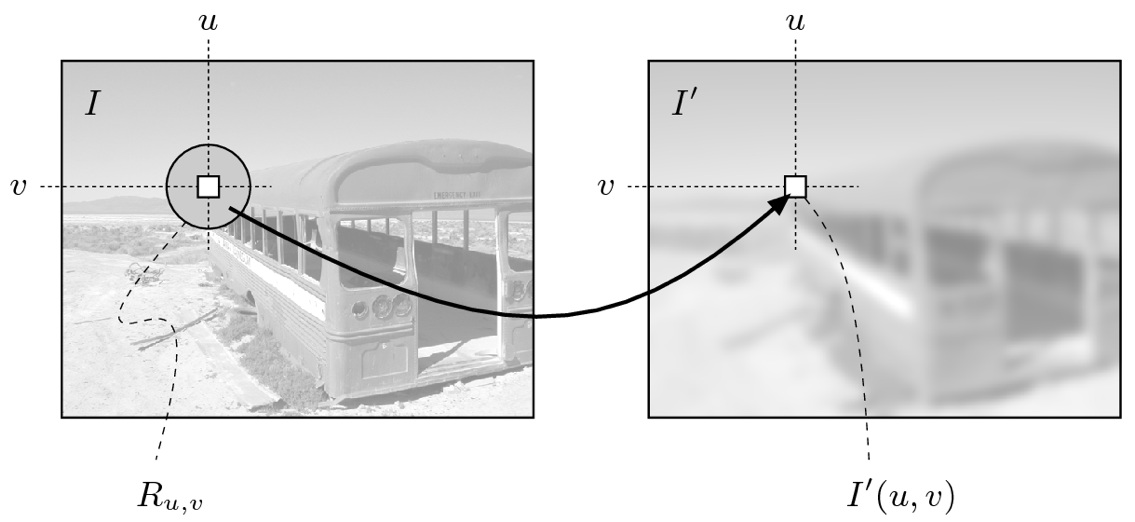
\includegraphics[scale=0.5]{localproc.png}
	\end{figure}
}

\frame
{
	\frametitle{What is local processing?}
	\selectlanguage{english}
	\begin{example}
		\begin{itemize}
			\item An image $I(u,v)$; a pixel $(u,v)$ and its neighborhood of $3\times 3 $ pixels
		\end{itemize}
		\centering
		\begin{figure}[!h]
			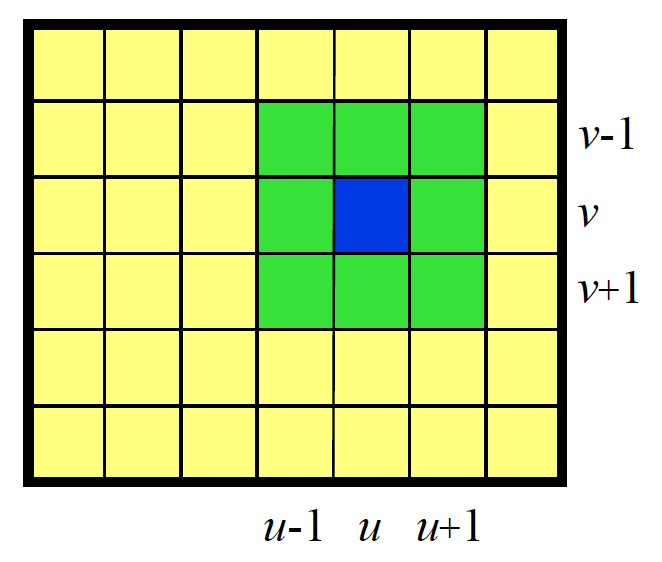
\includegraphics[scale=0.5]{neighborhood.png}
			\caption{Example of neighborhood}
		\end{figure}
	\end{example}
	
}

\frame
{
	\frametitle{What is local processing?}
	\begin{example}{Examples of some processing functions}
	\begin{itemize}
		\item Linear functions
		\begin{enumerate}
			\item Averaging function
			\item Shifting function
			\item Gaussian function
			\item Edge detecting function
		\end{enumerate}
		\item Non-linear functions
		\begin{enumerate}
			\item Median function
			\item Min function
			\item Max function
		\end{enumerate}
	\end{itemize}
	\end{example}
}
\frame
{
	\frametitle{What is local processing?}
	\begin{itemize}
		\item Example of an averaging function
	\end{itemize}
	\centering
	\begin{figure}[!h]
		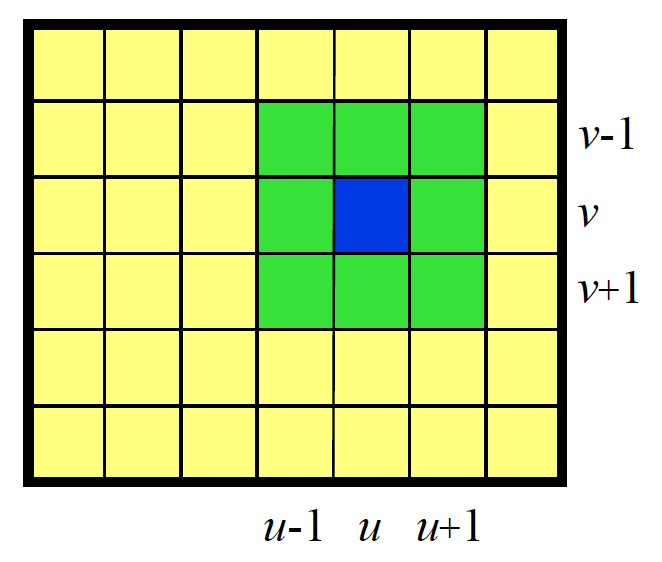
\includegraphics[scale=0.5]{neighborhood.png}
	\end{figure}
	\begin{equation*}
		I^{'}{(u,v)} = \frac{1}{9}\sum_{i=-1}^{1}{\sum_{j=-1}^{1}{I(u+i, v+j)}}
	\end{equation*}
	
}

\frame
{
	\frametitle{What is local processing?}
	\begin{itemize}
		\item Example of an averaging function
	\end{itemize}
	\centering
	\begin{figure}[!h]
		\begin{tabular}{cc}
			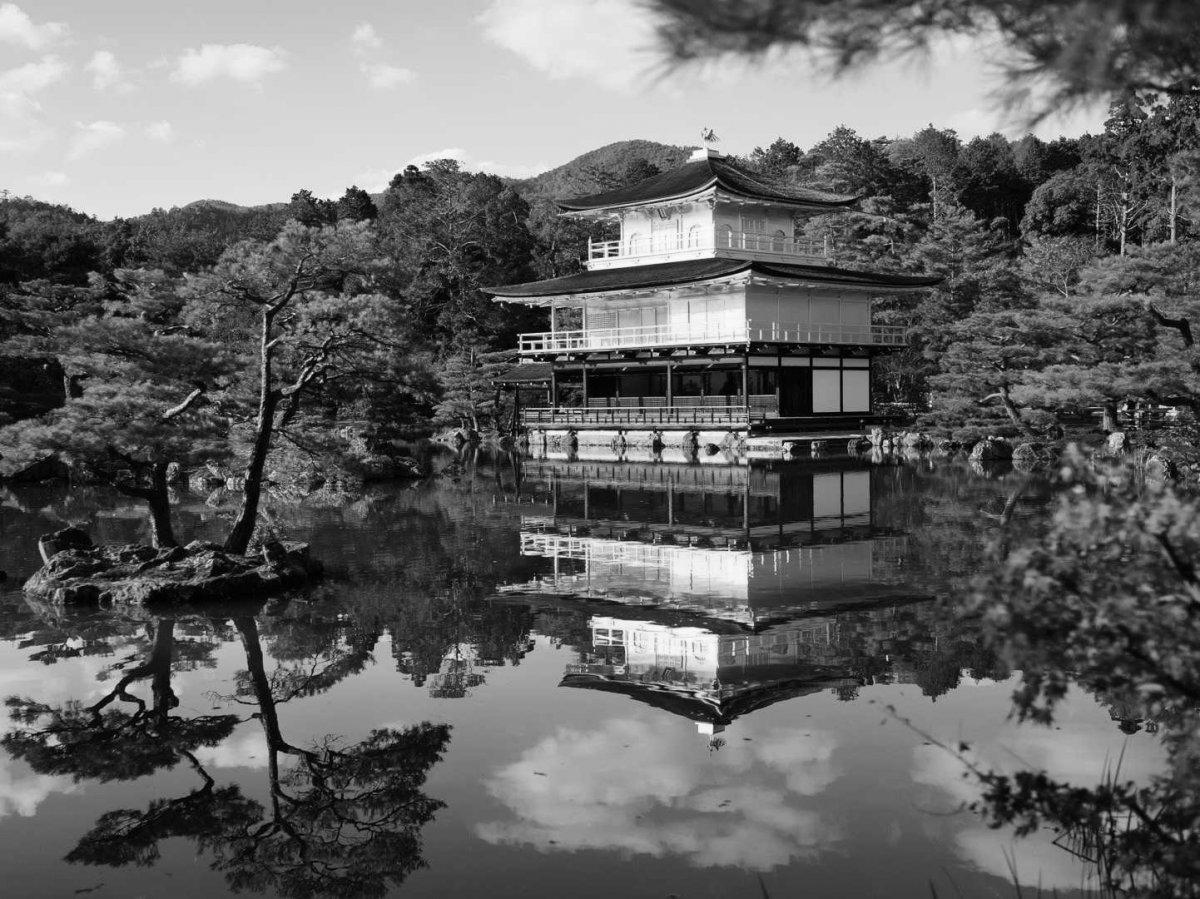
\includegraphics[scale=0.11]{kyoto_gray.jpg} &
			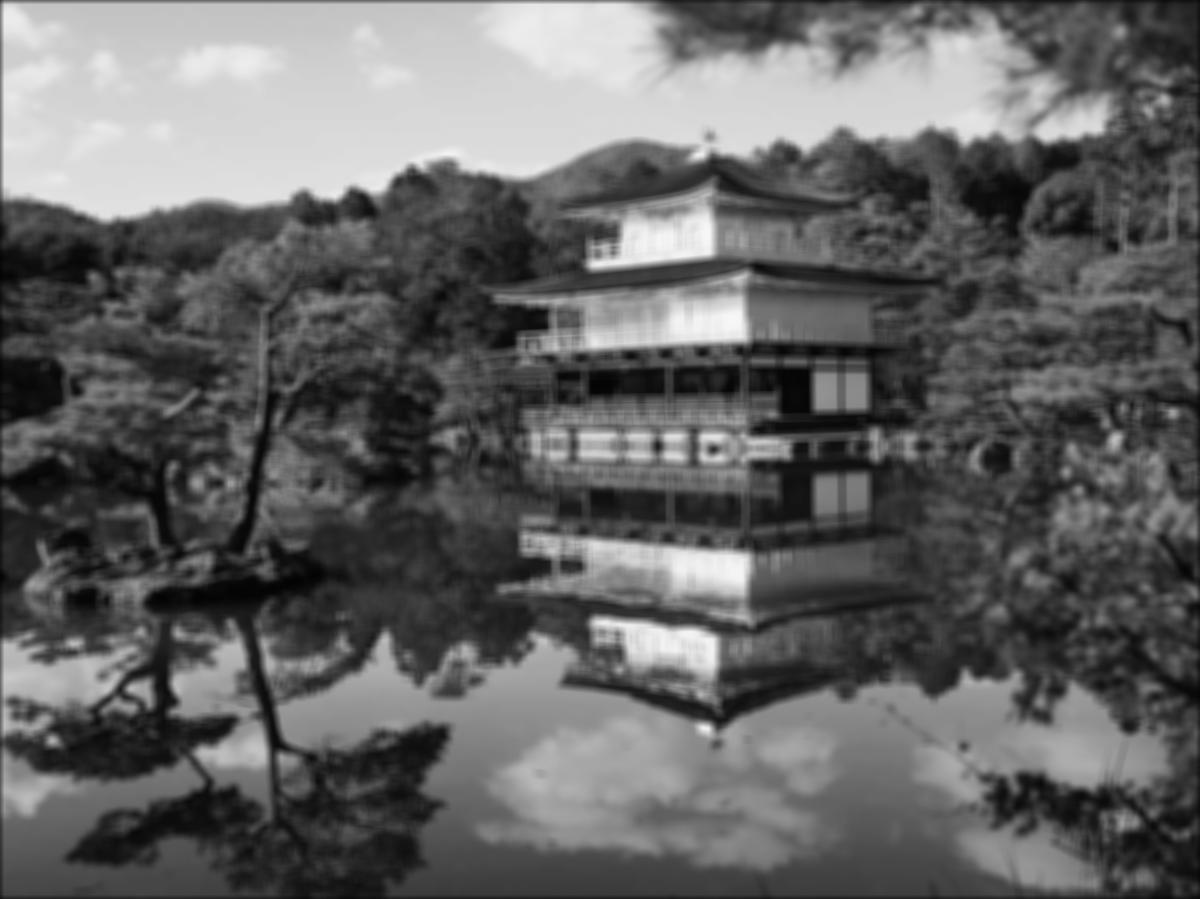
\includegraphics[scale=0.11]{kyoto_gray_smooth_9.jpg} \\
			Input image & Output image
		\end{tabular}
	\end{figure}

	\begin{itemize}
		\item The output image is obtained by averaging the input with neighborhood of $9 \times 9$ pixels.
	\end{itemize}
}
\frame
{
	\frametitle{What is local processing?}
	\begin{itemize}
		\item Example of an averaging function
	\end{itemize}
	\centering
	\begin{figure}[!h]
		\begin{tabular}{cc}
			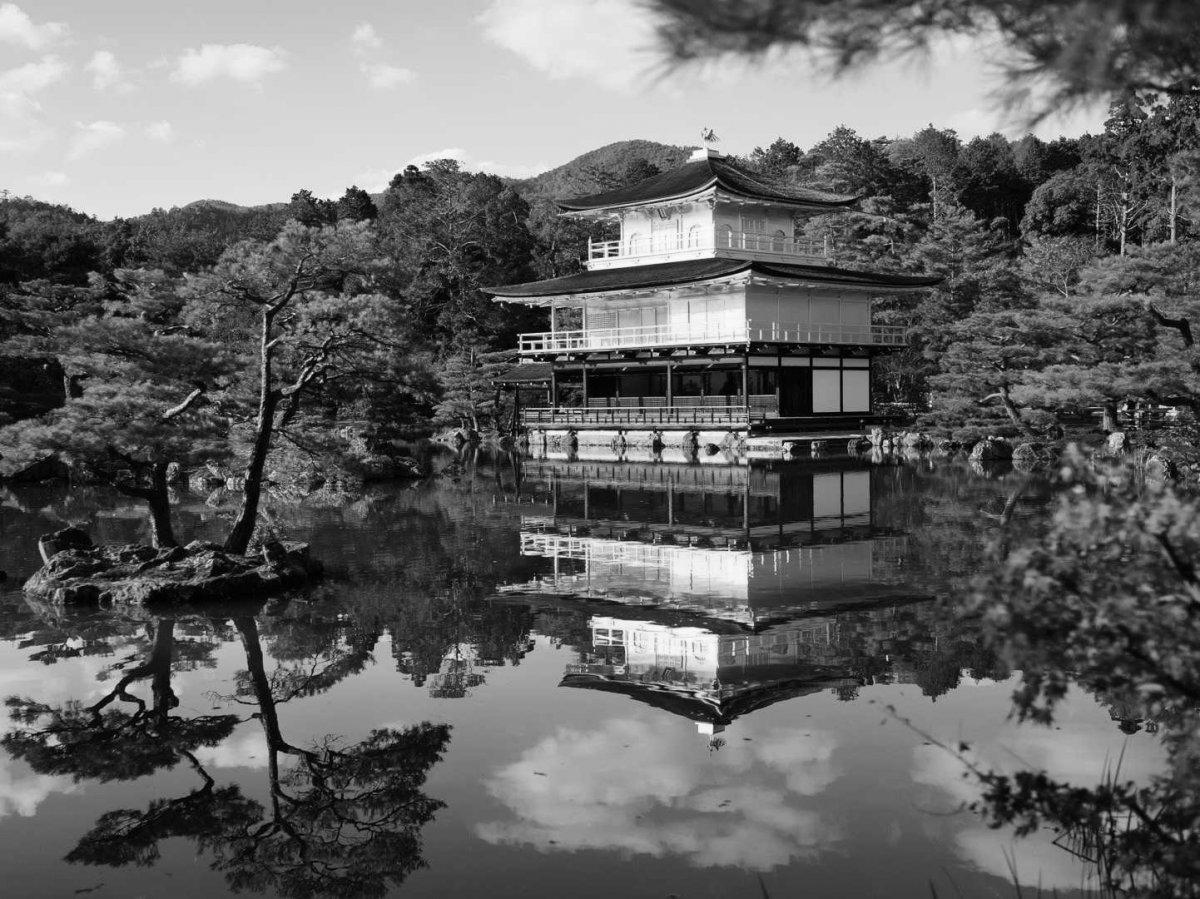
\includegraphics[scale=0.11]{kyoto_gray.jpg} &
			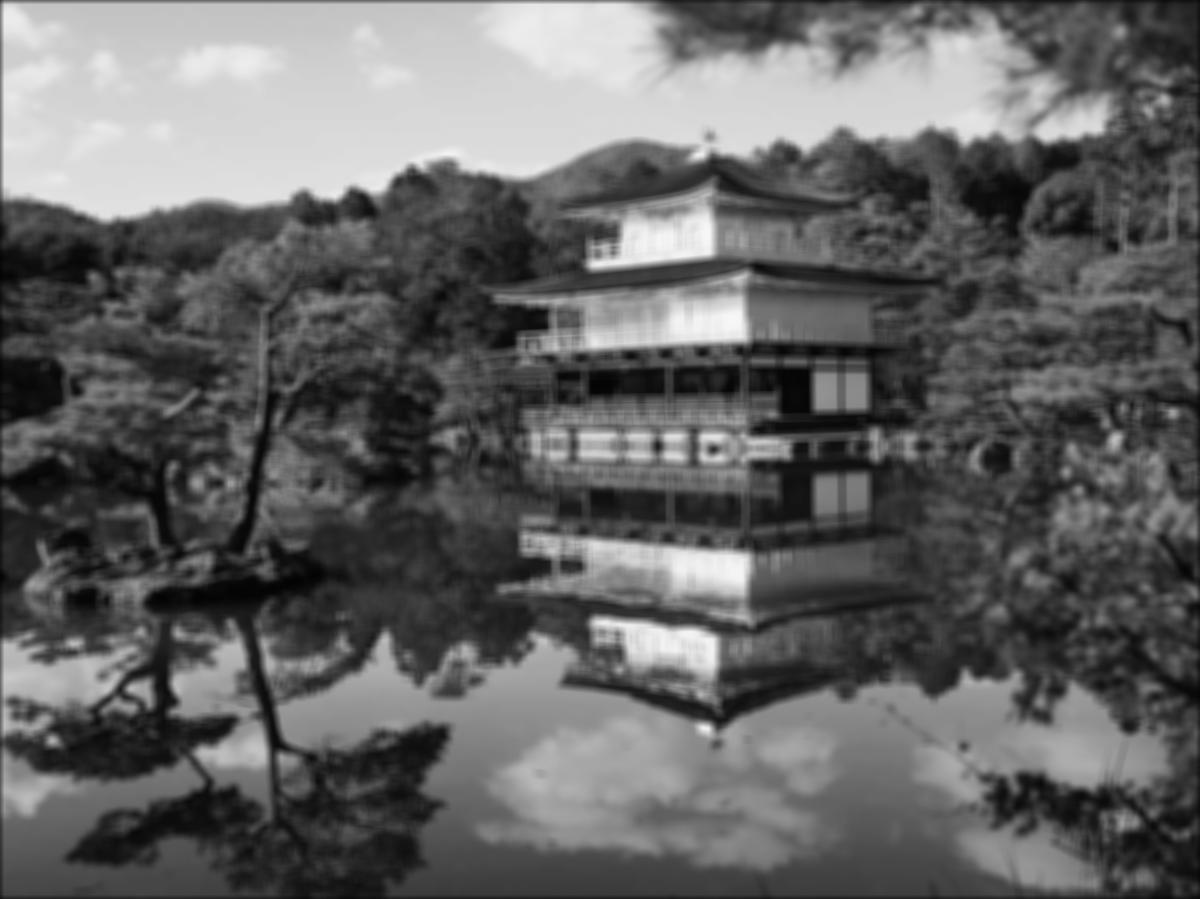
\includegraphics[scale=0.11]{kyoto_gray_smooth_9.jpg} \\
			Input image & Output image \\
						& blurred, smoothed
		\end{tabular}
	\end{figure}
	
	\begin{equation*}
	I^{'}{(u,v)} = \frac{1}{9\times 9}\sum_{i=-4}^{4}{\sum_{j=-4}^{4}{I(u+i, v+j)}}
	\end{equation*}
}
\frame
{
	\frametitle{What is local processing?}
	\begin{itemize}
		\item Example of a median function (a non-linear function)
	\end{itemize}
	\centering
	\begin{figure}[!h]
		\begin{tabular}{cc}
			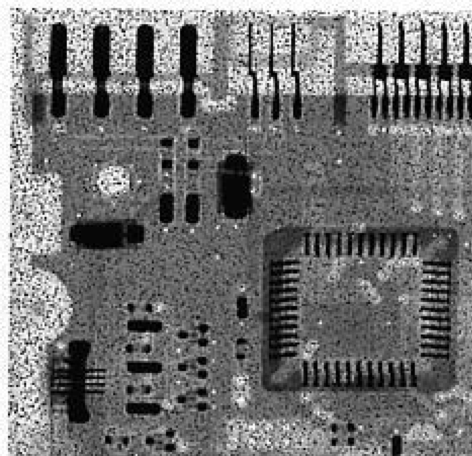
\includegraphics[scale=0.57]{image_salt_peper.png} &
			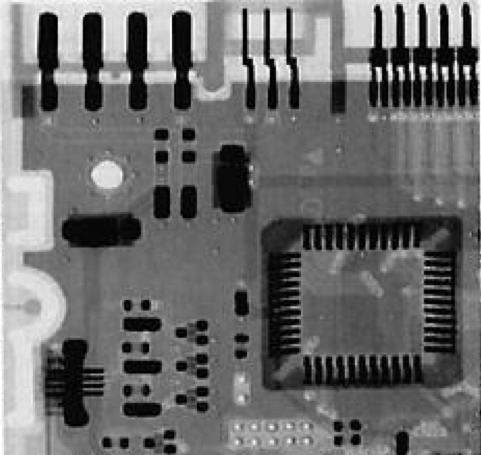
\includegraphics[scale=0.57]{image_salt_peper_denoise.png} \\
			Input image & Output image\\
				& Noises have been removed
		\end{tabular}
	\end{figure}
	
	\begin{itemize}
		\item The output image is obtained by computing the median value of a set of pixels in a neighborhood of $3 \times 3$ pixels.
	\end{itemize}
}


\section{Linear processing}
\frame
{
	\Huge
	\begin{center}
		\textcolor{blue}{\textbf{Linear processing function}}
	\end{center}
}

\subsection{Correlation}
\frame
{
	\frametitle{Mean function}
	Consider an averaging function on square window. In general, the window can have different size of each dimension. The output of the averaging is determined by.
	
	\begin{equation*} 
	\begin{split}
	I^{'}{(u,v)} &= \frac{1}{(2r+1) \times (2r+1)} \sum_{i=-r}^{r}{\sum_{j=-r}^{r}{I(u+i, v+j)}}
	\end{split}
	\end{equation*}
	
	$I^{'}(u,v)$ can be written as
	
	\begin{equation*} 
	\begin{split}
	I^{'}{(u,v)}	&= \sum_{i=-r}^{r}{\sum_{j=-r}^{r}{I(u+i, v+j).H_{corr}{(i,j)}}}
	\end{split}
	\end{equation*}
}
\frame
{
	\frametitle{Mean function}
	\begin{enumerate}
		\item $H_{corr}$ is a matrix of size $(2r+1) \times (2r+1)$ 
		\item $H_{corr} = \frac{1}{(2r+1) \times (2r+1)} M_{ones}$
		
		and,
		\item $M_{ones}$ : is an matrix of size $(2r+1) \times (2r+1)$ containing value 1 for all elements.
	
	\end{enumerate}
	
	\begin{example}
	Matrix for averaging pixels in a neighborhood of size $5 \times 5$, i.e., $r= 2$.
	$$
		H_{corr} = \frac{1}{5 \times 5} \times 
		\begin{bmatrix}
			1 & 1 & 1 & 1 & 1 \\
			1 & 1 & 1 & 1 & 1 \\
			1 & 1 & 1 & 1 & 1 \\
			1 & 1 & 1 & 1 & 1 \\
			1 & 1 & 1 & 1 & 1 \\
		\end{bmatrix}
	$$
	\end{example}
}
\frame
{
	\frametitle{From averaging function to others}
	\begin{block}{A way to construct other linear processing functions}
		If one changes $H_{corr}$ to other kinds of matrix, he obtains other linear function.
	\end{block}
	
	\begin{example}
	Edge detecting function (Sobel)
	$$
		H_{corr} = 
		\begin{bmatrix}
			1 & 0 & -1 \\
			2 & 0 & -2 \\
			1 & 0 & -1 \\
		\end{bmatrix}
		\quad 
		H_{corr} = 
		\begin{bmatrix}
			1 & 2 & 1 \\
			0 & 0 & 0 \\
			-1 & -2 & -1 \\
		\end{bmatrix}
	$$
	
	Shifting function
	$$
	H_{corr} = 
	\begin{bmatrix}
		0 & 0 & 0 \\
		0 & 0 & 1 \\
		0 & 0 & 0 \\
	\end{bmatrix}
	$$
	\end{example}
}


\frame
{
	\frametitle{Correlation}
	
	\begin{block}{Definition}
		Input data:
		\begin{enumerate}
			\item Input image, $I(u,v)$
			\item Matrix $H_{corr}{(i,j)}$ of size $(2r+1) \times (2r+1)$. In general, the size on two dimensions maybe different.
		\end{enumerate}
		\textbf{Correlation} is defined as follows:
		\begin{equation*} 
		\begin{split}
		I_{corr}^{'}{(u,v)} &= \sum_{i=-r}^{r}{\sum_{j=-r}^{r}{I(u+i, v+j).H_{corr}{(i,j)}}}
		\end{split}
		\end{equation*}
	\end{block}
}


\frame
{
	\frametitle{Correlation: How does it works?}
	\selectlanguage{english}
	\begin{figure}[!h]
		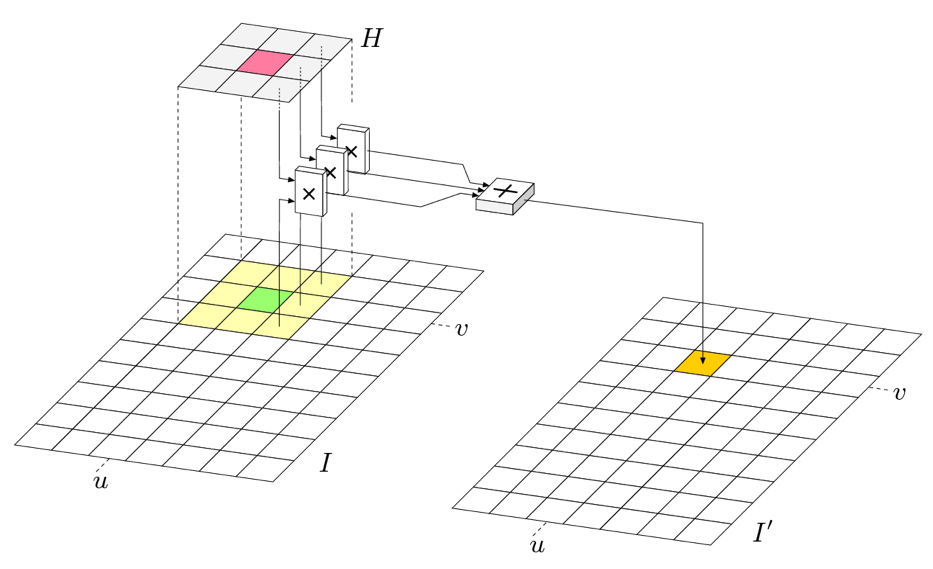
\includegraphics[scale=0.57]{correlation.png}
		\caption{Method for computing the correlation for one pixel}
	\end{figure}
}

\frame
{
	\frametitle{Correlation: How does it works?}
	\selectlanguage{english}
	\begin{block}{A computation process}
		For each pixel $(u,v)$ on the output image, do:
		\begin{enumerate}
			\item \textbf{Place} matrix $H_{corr}$ centered at the corresponding pixel, i.e., pixel $(u,v)$, on the input image
			\item \textbf{Multiply} coefficients in matrix $H_{corr}$ with the underlying pixels on the input image.
			\item \textbf{Compute} the sum of all the resulting products in the previous step.
			\item \textbf{Assign} the sum to the $I^{'}(u,v)$.
		\end{enumerate}
	
	\end{block}
}


\subsection{Convolution}
\frame
{
	\frametitle{Convolution}
	\selectlanguage{english}
		
	\begin{block}{Definition}
		Input data:
		\begin{enumerate}
			\item Input image, $I(u,v)$
			\item Matrix $H_{conv}$ of size $(2r+1) \times (2r+1)$. In general, the size on two dimensions maybe different.
		\end{enumerate}
		\textbf{Convolution} is defined as follows:
		\begin{equation*} 
		\begin{split}
		I_{conv}^{'}{(u,v)} &= \sum_{i=-r}^{r}{\sum_{j=-r}^{r}{I(u-i, v-j).H_{conv}{(i,j)}}}
		\end{split}
		\end{equation*}
	\end{block}
}

\frame
{
	\frametitle{Convolution}
	\selectlanguage{english}
	
	\begin{block}{Natation}
		\begin{itemize}
			\item \alert{Operator *} is used to denote the convolution between image $I$ and matrix $H_{conv}$
			\item That is
			
			\begin{equation*} 
			\begin{split}
			I_{conv}^{'}{(u,v)} &= I * H_{conv} \\
				&= \sum_{i=-r}^{r}{\sum_{j=-r}^{r}{I(u-i, v-j).H_{conv}{(i,j)}}}
			\end{split}
			\end{equation*}
		\end{itemize}
		
		
	\end{block}
}
\frame
{
	\frametitle{Convolution}
	\selectlanguage{english}
	
	\begin{alertblock}{Attention!}
		\begin{itemize}
			\item When $I$ is an gray image, both of $I$ and $H_{conv}$ are matrices.
			\item However,  $I * H_{conv}$ is convolution between $I$ and $H_{conv}$, \textbf{instead of matrix multiplication}!
	
	\end{itemize}
	
	
	\end{alertblock}
}


\frame
{
	\frametitle{Convolution and Correlation}
	\selectlanguage{english}
	
	\begin{block}{Mathematics}
		\begin{equation*} 
		\begin{split}
		I_{conv}^{'}{(u,v)} &= \sum_{i=-r}^{r}{\sum_{j=-r}^{r}{I(u-i, v-j).H_{conv}{(i,j)}}} \\
		I_{corr}^{'}{(u,v)} &= \sum_{i=-r}^{r}{\sum_{j=-r}^{r}{I(u+i, v+j).H_{corr}{(i,j)}}}
		\end{split}
		\end{equation*}
	\end{block}
	In mathematics, convolution and correlation are different in the \textbf{sign} of $i$ and $j$ inside of $I(u+i, v+j)$ and $I(u-i, v-j)$
}
\frame
{
	\frametitle{Convolution and Correlation}
	\selectlanguage{english}
	
	\begin{block}{Convolution to Correlation}
		\begin{itemize}
			\item Let $s=-i$ and $t=-j$ 
			\item We have
		\end{itemize}
		\begin{equation*} 
		\begin{split}
		I_{conv}^{'}{(u,v)} &= \sum_{i=-r}^{r}{\sum_{j=-r}^{r}{I(u-i, v-j).H_{conv}{(i,j)}}} \\
				&= \sum_{i=-r}^{r}{\sum_{j=-r}^{r}{I(u+s, v+t).H_{conv}{(-s,-t)}}} 
		\end{split}
		\end{equation*}
	\end{block}
	\begin{alertblock}{$H_{conv}{(-s,-t)}$ from $H_{conv}{(i,j)}$}
		$H_{conv}{(-s,-t)}$ can be obtained from $H_{conv}{(i,j)}$ by either
			\begin{itemize}
				\item \textbf{Flipping} $H_{conv}{(i,j)}$ on x and then on y axis
				\item \textbf{Rotating} $H_{conv}{(i,j)}$ around its center $180^0$
			\end{itemize}
	\end{alertblock}
	
}
\frame
{
	\frametitle{Convolution and Correlation}
	\selectlanguage{english}

	
	\begin{example}
		Demonstration of rotation and flipping.
		
		$$
		H = 
		\begin{bmatrix}
		\textcircled{1} & 2 & 3 \\
		4 & 5 & 6 \\
		7 & 8 & 9 \\
		\end{bmatrix}
		\quad
		H_{flipped\_x} = 
		\begin{bmatrix}
		3 & 2 & \textcircled{1} \\
		6 & 5 & 4 \\
		9 & 8 & 7 \\
		\end{bmatrix}
		$$
		$H_{flipped\_x}$ is obtained from $H$ by flipping $H$ on x-axis.
		
		After flipping $H_{flipped\_x}$ around y axis
		$$
		H_{flipped\_xy} = 
		\begin{bmatrix}
		9 & 8 & 7 \\
		6 & 5 & 4 \\
		3 & 2 & \textcircled{1} \\
		\end{bmatrix}
		$$
		
		$H_{flipped\_xy}$ can obtained from $H$ by rotating $H$	$180^0$ around $H$'s center.
		\end{example}
}

\frame
{
	\frametitle{Convolution and Correlation}
	\selectlanguage{english}
	
	\begin{block}{Correlation to Convolution}
	\begin{itemize}
	\item Let $s=-i$ and $t=-j$ 
	\item We have
	\end{itemize}
	\begin{equation*} 
	\begin{split}
	I_{corr}^{'}{(u,v)} &= \sum_{i=-r}^{r}{\sum_{j=-r}^{r}{I(u+i, v+j).H_{corr}{(i,j)}}} \\
	&= \sum_{i=-r}^{r}{\sum_{j=-r}^{r}{I(u-s, v-t).H_{corr}{(-s,-t)}}} 
	\end{split}
	\end{equation*}
	\end{block}
	\begin{alertblock}{$H_{corr}{(-s,-t)}$ from $H_{corr}{(i,j)}$}
	$H_{corr}{(-s,-t)}$ can be obtained from $H_{corr}{(i,j)}$ by either
	\begin{itemize}
	\item \textbf{Flipping} $H_{corr}{(i,j)}$ on x and then on y axis
	\item \textbf{Rotating} $H_{corr}{(i,j)}$ around its center $180^0$
	\end{itemize}
	\end{alertblock}
	
}
\frame
{
	\frametitle{Convolution-Correlation Conversion}
	\selectlanguage{english}
	\begin{alertblock}{Relationship}
	\begin{enumerate}
		
		\item Convolution can be computed by correlation and vice versa.
		
		\item For example, convolution can be computed by correlation by: first, \alert{(a)} rotating the matrix $180^0$ and then \alert{(b)} computing the correlation between the rotated matrix with the input image.
		
	\end{enumerate}
	
	\end{alertblock}
}

\frame
{
	\frametitle{Convolution: How does it works?}
	\selectlanguage{english}
	\begin{block}{A Computation process}
		\begin{enumerate}
			\item \textbf{Rotate} matrix $H_{conv}$ around its center $180^0$ to obtain $H_{corr}$
		\end{enumerate}
		For each pixel $(u,v)$ on the output image, do:
		\begin{enumerate}
			\item \textbf{Place} matrix $H_{corr}$ centered at the corresponding pixel, i.e., pixel $(u,v)$, on the input image
			\item \textbf{Multiply} coefficients in matrix $H_{corr}$ with the underlying pixels on the input image.
			\item \textbf{Compute} the sum of all the resulting products in the previous step.
			\item \textbf{Assign} the sum to the $I^{'}(u,v)$.
		\end{enumerate}
		
	\end{block}
}
\frame
{
	\frametitle{MATLAB's function}
	\selectlanguage{english}
	\begin{example}
		MATLAB's functions supports correlation and convolution
		\begin{enumerate}
			\item \alert{\textbf{corr2}}
			\item \alert{\textbf{xcorr2}}
			\item \alert{\textbf{conv2}}
			\item \alert{\textbf{filter2}}
			\item \alert{\textbf{imfilter}}
		\end{enumerate}
			MATLAB's function supports creating special matrix
			\begin{enumerate}
				\item \alert{\textbf{fspecial}}
			\end{enumerate}
	\end{example}
}


\subsection{Linear Filtering}
\frame
{
	\frametitle{Linear Filtering}
	\selectlanguage{english}
	\begin{block}{Definition}
		Linear filtering is a process of applying the \alert{\textbf{convolution or the correlation}} between an matrix $H$ to input image $I(u,v)$.
	\end{block}
	\begin{block}{Model of a filter system}
		\begin{figure}[!h]
			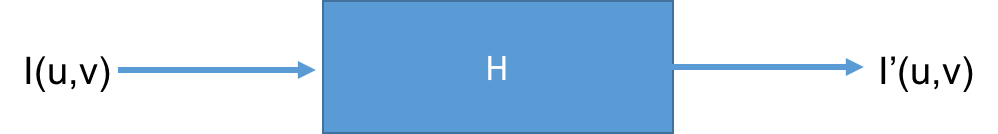
\includegraphics[scale=0.57]{filtersys.png}
			\caption{Filter image $I(u,v)$ with matrix $H$ to obtain $I^{'}(u,v)$} 
		\end{figure}
		
		\centering
		$I^{'}(u,v) =  I(u,v)*H(i,j)$
	\end{block}
}
\frame
{
	\frametitle{Filter's kernel}
	\selectlanguage{english}
	\begin{block}{Definition}
		In filtering, matrix $H$ is called the filter's kernel.
	\end{block}
	\begin{block}{Other names of $H$}
		\begin{itemize}
			\item Filter's kernel
			\item Window
			\item Mask
			\item Template
			\item Matrix
			\item Local region
		\end{itemize}
	\end{block}
}
\subsection{Popular Linear Filter}
\frame
{
	\frametitle{Popular Linear Filter: Mean filter}
	\selectlanguage{english}
	\begin{example}
		Mean filter's kernel
		\begin{itemize}
			\item General case:
		\end{itemize}
		$$
		H_{corr} = \frac{1}{(2r+1)^2} \times 
		\begin{bmatrix}
		1 & 1 & ... & 1 & 1 \\
		1 & 1 & ... & 1 & 1 \\
		... & ... & ... & ... & ... \\
		1 & 1 & ... & 1 & 1 \\
		1 & 1 & ... & 1 & 1 \\
		\end{bmatrix}_{(2r+1) \times (2r+1)}
		$$
	\end{example}
}

\frame
{
	\frametitle{Popular Linear Filter: Mean filter}
	\selectlanguage{english}
	\begin{figure}
		\begin{tabular}{cc}
			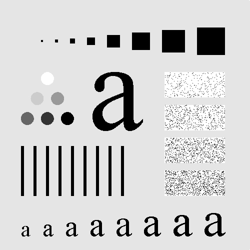
\includegraphics[scale=0.53]{char.png} &
			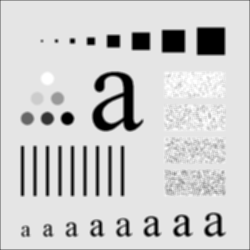
\includegraphics[scale=0.53]{char_mean_3_3.png} \\
			Original image & Filtered with $H$'s size: $3 \times 3$
		\end{tabular}
	\end{figure}
}

\frame
{
	\frametitle{Popular Linear Filter: Mean filter}
	\selectlanguage{english}
	\begin{figure}
		\begin{tabular}{cc}
			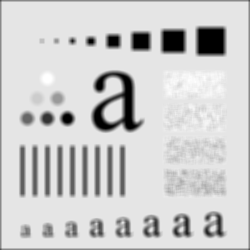
\includegraphics[scale=0.53]{char_mean_5_5.png} &
			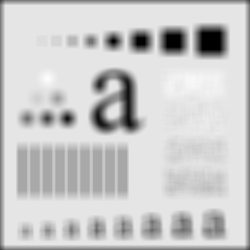
\includegraphics[scale=0.53]{char_mean_11_11.png} \\
			Filtered with $H$'s size: $5 \times 5$ & Filtered with $H$'s size: $11 \times 11$ 
		\end{tabular}
	\end{figure}
}

\frame
{
	\frametitle{Popular Linear Filter: Gaussian filter}
	\selectlanguage{english}
	\begin{block}{2D-Gaussian Function}
		\begin{equation*}
		\begin{split}
				G(x,y, \sigma) &= \frac{1}{2\pi{\sigma}^2}  exp({-\frac{x^2 + y^2}{{2\sigma}^2}})
		\end{split}
		\end{equation*}
	\end{block}
	\begin{figure}
		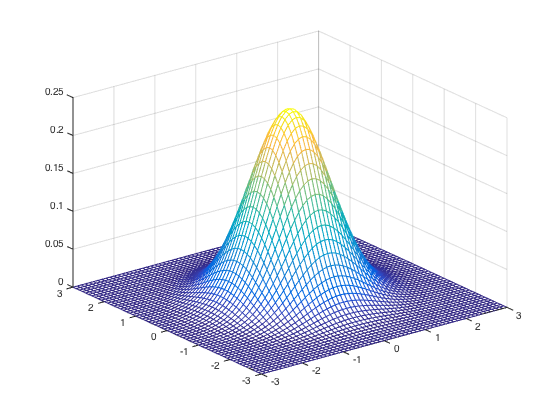
\includegraphics[scale=0.3]{gaussian.png}
		\caption{2D-Gaussian Function}
	\end{figure}
}

\frame
{
	\frametitle{Popular Linear Filter: Gaussian filter}
	\selectlanguage{english}
	\begin{example}
		\begin{itemize}
			\item $H$'s size is $3 \times 3$
			\item $\sigma = 0.5$
		\end{itemize}
		$$
		H = 
		\begin{bmatrix}
		0.0113   & 0.0838  &  0.0113\\
		0.0838   & 0.6193  &  0.0838\\
		0.0113   & 0.0838  &  0.0113
		\end{bmatrix}
		$$
		\begin{itemize}
			\item $H$'s size is $5 \times 5$
			\item $\sigma = 0.5$
		\end{itemize}
		$$
		H = 
		\begin{bmatrix}
		0.0000  &  0.0000  &  0.0002  &  0.0000  &  0.0000\\
		0.0000  &  0.0113  &  0.0837  &  0.0113  &  0.0000\\
		0.0002  &  0.0837  &  0.6187  &  0.0837  &  0.0002\\
		0.0000  &  0.0113  &  0.0837  &  0.0113  &  0.0000\\
		0.0000  &  0.0000  &  0.0002  &  0.0000  &  0.0000
		\end{bmatrix}
		$$
	\end{example}
}
\frame
{
	\frametitle{Popular Linear Filter: Gaussian filter}
	\selectlanguage{english}
	\begin{figure}
		\begin{tabular}{cc}
			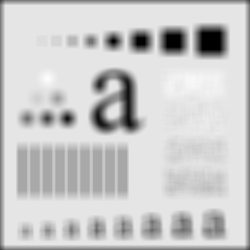
\includegraphics[scale=0.53]{char_mean_11_11.png} &
			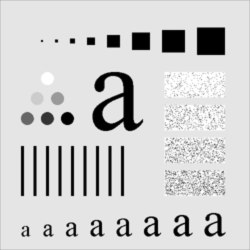
\includegraphics[scale=0.53]{char_gaussian_11_11_05.png} \\
			Filtered with Mean filter  & Filtered with Gaussian filter \\
			$H$'s size: $11 \times 11$ & $H$'s size: $11 \times 11$ \\
									& 	$\sigma =0.5$
		\end{tabular}
	\end{figure}
}

\frame
{
	\frametitle{Popular Linear Filter: Shifting filter}
	\selectlanguage{english}
	\begin{example}
		\begin{itemize}
			\item In order to shift pixel $(u,v)$ to $(u-2, v+2)$, use the following kernel
		\end{itemize}
		$$
		H = 
		\begin{bmatrix}
		0 & 0 & 0 & 0 & 1\\
		0 & 0 & 0 & 0 & 0\\
		0 & 0 & 0 & 0 & 0\\
		0 & 0 & 0 & 0 & 0\\
		0 & 0 & 0 & 0 & 0\\
		\end{bmatrix}
		$$
		
	\end{example}
}

\frame
{
	\frametitle{Popular Linear Filter: Shifting filter}
	\selectlanguage{english}
	\begin{figure}
		\begin{tabular}{cc}
			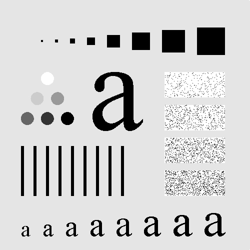
\includegraphics[scale=0.53]{char.png} &
			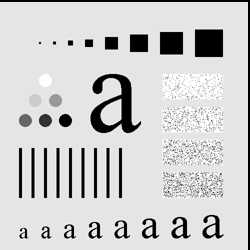
\includegraphics[scale=0.53]{char_shifted_2_2.png} \\
			Original image & Shifted with $d=[-2, 2]$ 
		\end{tabular}
	\end{figure}
}

\subsection{Convolution's Properties}
\frame
{
	\frametitle{Convolution's Properties}
	\selectlanguage{english}
	\begin{block}{Commutativity:}
		\centering
		$I * H = H * I$
	\end{block}
	\begin{alertblock}{Meaning}
		\begin{enumerate}
			\item This means that we can think of the image as the kernel and the kernel as the image and get the same result. 
			
			\item In other words, we can leave the image fixed and slide the kernel or leave the kernel fixed and slide the image.
		\end{enumerate}		
		
	\end{alertblock}
}

\frame
{
	\frametitle{Convolution's Properties}
	\selectlanguage{english}
	\begin{block}{Associativity:}
		\centering
		$(I * H_{1})*H_{2} =I * (H_{1}*H_{2})$
	\end{block}
	\begin{alertblock}{Meaning}
		\begin{enumerate}
			\item This means that we can apply $H_{1}$ to $I$ followed by $H_{2}$, or we can convolve the kernel $H_{2} * H_{1}$  and then apply the resulting kernel to $I$.
		\end{enumerate}		
		
	\end{alertblock}
}
\frame
{
	\frametitle{Convolution's Properties}
	\selectlanguage{english}
	\begin{block}{Linearity:}
		\centering
		$(\alpha .I)* H = \alpha. (I * H)$
		
		$(I_{1} + I_{2}) * H = I_{1} * H + I_{2}*H$
		
	\end{block}
	\begin{alertblock}{Meaning}
		\begin{enumerate}
			\item This means that we can multiply an image by a constant before or after convolution, and we can add two images before or after convolution and get the same results. 
		\end{enumerate}		
		
	\end{alertblock}
}
\frame
{
	\frametitle{Convolution's Properties}
	\selectlanguage{english}
	\begin{block}{Shift-Invariance}
		Let $S$ be an operator that shifts an image I:
		\centering
		$S(I)(u,v) = I(u+a, v+b)$
		
		
		\flushleft Then,
		
		\centering
		$S(I*H) = S(I)*H$
		
	\end{block}
	\begin{alertblock}{Meaning}
		
		\begin{enumerate}
			\item This means that we can convolve $I$ and $H$ and then shift the result, or we can shift $I$ and then convolve it with $H$.
		\end{enumerate}		
		
	\end{alertblock}
}

\frame
{
	\frametitle{Convolution's Properties}
	\selectlanguage{english}
	\begin{block}{Separability}
		A kernel H is called separable if it can be broken down into the convolution of two kernels:
		
		\centering $H = H_{1} * H_{2}$
		
		\flushleft More generally, we might have:
		
		\centering $H = H_{1} * H_{2}* ... * H_{n}$
	\end{block}
}


\frame
{
	\frametitle{Convolution's Properties}
	\selectlanguage{english}
	\begin{example}
		$$
		H_{x} = 
		\begin{bmatrix}
		1 & 1 & 1 & 1 & 1
		\end{bmatrix}
		\quad
		H_{y} = 
		\begin{bmatrix}
		1 \\ 1 \\ 1
		\end{bmatrix}
		$$
		
		Then,
		$$
		H_{x}  = H_{x} * H_{y} = 
		\begin{bmatrix}
			1 & 1 & 1 & 1 & 1\\
			1 & 1 & 1 & 1 & 1\\
			1 & 1 & 1 & 1 & 1
		\end{bmatrix}
		$$
		
	\end{example}
	
}
\frame
{
	\frametitle{Processing at the boundary of image}
	\selectlanguage{english}
	
	\begin{figure}[!h]
		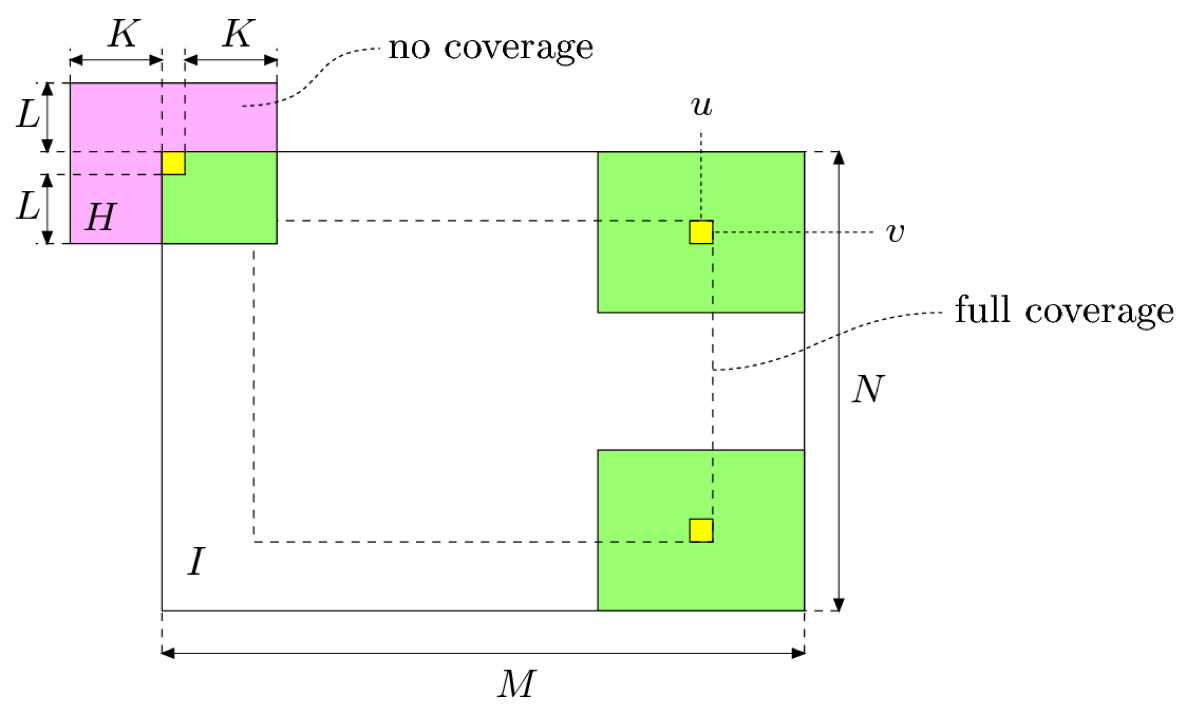
\includegraphics[scale=0.57]{boundary_effect.png}
		\caption{Without any special consideration, the processing is invalid at boundary pixels} 
	\end{figure}

}
\frame
{
	\frametitle{Processing at the boundary of image}
	\selectlanguage{english}
	
	\begin{block}{Methods for processing boundary pixels}
		\begin{enumerate}
			\item \textbf{Cropping}:do not process boundary pixels. Just obtain a smaller output image by cropping the output image.
			\item \textbf{Padding}: pad a band of pixels (with zeros) to the boundary of input image. Perform the processing and the crop to get the output image.
			\item \textbf{Extending}: copy pixels on the boundary to outside to get a new image. Perform the processing and the crop to get the output image.
			\item \textbf{Wrapping}: reflect pixels on the boundary to outside to get a new image. Perform the processing and the crop to get the output image.
			
		\end{enumerate} 
	\end{block}
	
}

\frame
{
	\frametitle{Convolution's implementation}
	\selectlanguage{english}
	
	\begin{block}{Methods for implementing convolution and correlation}
		\begin{enumerate}
			\item \textbf{In space domain}:
				\begin{itemize}
					\item Use sliding widow technique
					\item Use speed-up methods for special cases
				\end{itemize}
			\item \textbf{In frequency domain}: will be presented in next chapter
			
		\end{enumerate} 
	\end{block}
	
}
\subsection{Convolution's implementation}
\frame
{
	\frametitle{Convolution's implementation}
	\selectlanguage{english}
	
	\begin{alertblock}{Sliding window technique for correlation}
		For each pixel $(u,v)$ on the output image, do:
		\begin{enumerate}
			\item \textbf{Place} matrix $H_{corr}$ centered at the corresponding pixel, i.e., pixel $(u,v)$, on the input image
			\item \textbf{Multiply} coefficients in matrix $H_{corr}$ with the underlying pixels on the input image.
			\item \textbf{Compute} the sum of all the resulting products in the previous step.
			\item \textbf{Assign} the sum to the $I^{'}(u,v)$.
		\end{enumerate}
	\end{alertblock}
	Convolution can be computed by rotating the kernel $180^0$ followed by the above algorithm.
}
\frame
{
	\frametitle{Convolution's complexity}
	\selectlanguage{english}
	\begin{block}{Computational Complexity of sliding window technique}
		\begin{itemize}
			\item Input image $I$ has size $N \times M$
			\item Kernel's size is $(2r+1) \times (2r+1)$
			\item Then, the number of operations is directly proportional to: $MN[(2r+1)^2 + (2r+1)^2 -1]$.
			\item \alert{\textbf{The computational complexity is $O(MNr^2)$}}
		\end{itemize}
		
	\end{block}
	\begin{alertblock}{Attention!}
		\begin{itemize}
			\item The cost for computing convolution and correlation is \alert{directly proportional} to the kernel's size!
			\item The filtering process will be slower if the kernel's size is bigger.
			\item The computational cost of the implementation in frequency domain is independent with the kernel's size.
		\end{itemize}
	\end{alertblock}
	
}
\frame
{
	\frametitle{Convolution's complexity}
	\selectlanguage{english}
	\begin{example}
		To shift an image $I$ to left 10 pixels. We can apply the following methods:
		\begin{enumerate}
			\item \textbf{Method 1:} Filter $I$ with a shifting kernel of size $21 \times 21$.
			\item \textbf{Method 2:} Apply 10 times shifting kernel of size $3 \time 3$.
		\end{enumerate}
		Which method can result better computation cost?
		
	\end{example}
	\begin{block}{Answer}
	Number of operations for each method is proportional to:
	\begin{enumerate}
		\item \textbf{Method 1:} $MN \times (21^2) = 441MN$
		\item \textbf{Method 2:} $10 \times MN \times(3^2) = 90MN$
	\end{enumerate}
	Method 2 is better than Method 1!
	
	\end{block}

	
}


\frame
{
	\frametitle{Convolution's complexity}
	\selectlanguage{english}
	Because, we have
	\begin{block}{Associativity:}
		\centering
		$(I * H_{1})*H_{2} =I * (H_{1}*H_{2})$
	\end{block}
	
	\begin{alertblock}{So, we can save the computational cost by using separability}
		If we can separate a kernel H into two smaller kernels $H = H_{1} * H_{2}$, then it will often be cheaper to apply $H_{1}$ followed by $H_{2}$, rather than $H$.
	\end{alertblock}
}
\frame
{
	\frametitle{Convolution's complexity}
	\selectlanguage{english}
	\begin{example}
		Kernel $H$ can be decomposed into $H = H_{1} *H_{2}$, as follows:
		$$
		H_{1} = 
		\begin{bmatrix}
			1 \\ 2 \\ 1
		\end{bmatrix}
		\quad
		H_{2} = 
		\begin{bmatrix}
			-1 & 0 & 1	
		\end{bmatrix}
		$$
		
		$$
		H  = H_{1} * H_{2} = 
		\begin{bmatrix}
			-1 & 0 & 1\\
			-2 & 0 & 2\\
			-1 & 0 & 1
		\end{bmatrix}
		$$
		Using associativity, we can filter image $I$ with $H$ by either
		\begin{enumerate}
			\item \textbf{Method 1:} $I' = I*H$
			\item \textbf{Method 2:} $I' = (I*H_{1})*H_{2}$
		\end{enumerate}
		Which method is better?
	\end{example}	
}
\frame
{
	\frametitle{Convolution's complexity}
	\selectlanguage{english}
	\begin{block}{Answer}
		Number of operations for each method is proportional to:
		\begin{enumerate}
			\item \textbf{Method 1:} $MN \times (3^2) = 9MN$
			\item \textbf{Method 2:} $(MN \times 3) + (MN \times 3) = 6MN$
		\end{enumerate}
		Method 2 is better than Method 1!
	\end{block}
}
\frame
{
	\frametitle{Convolution's implementation}
	\selectlanguage{english}
	\begin{alertblock}{Special cases}
		\begin{enumerate}
			\item \textbf{Separability:} In the case that kernel filter $H$ can be separated into smaller kernels. Consecutively apply smaller kernels to the input image can reduce the computation time, as shown in previous slide.
			\item \textbf{Box Filtering: } Kernel's coefficients of box filter are equal (value 1). So, we can use \textbf{integral image} to speed up.
		\end{enumerate}

	\end{alertblock}
}
\frame
{
	\frametitle{Convolution's implementation: Integral image}
	\selectlanguage{english}
	
	\tikzstyle{pointer} = [draw, thin, fill=blue!20, minimum height=2em, minimum width=4em]
	\tikzstyle{value} = [draw, thin, minimum height=2em, minimum width=4em]
	
	\tikzstyle{innerWhite} = [semithick, white,line width=1.4pt, shorten >= 4.5pt]
	
	\textbf{CASE 1: 1D-array}
	\begin{itemize}
		\item Input data: array $A[i]$, for $i\in [1,n]$
		\begin{itemize}
			\item The first element, $A[0]$, is not used
		\end{itemize}
	\end{itemize}
	
		\begin{tikzpicture}
		\begin{scope}[start chain=1 going right, node distance=-0.1mm]
		\node [on chain=1,tmtape] (n0) {};
		\node [on chain=1,tmtape] (n1) {3};
		\node [on chain=1,tmtape] (n2) {8};
		\node [on chain=1,tmtape] (n3) {2};
		\node [on chain=1,tmtape] (n4) {6};
		\node [on chain=1,tmtape] (n5) {9};
		\node [on chain=1,tmtape] (n6) {7};
		\node [on chain=1,tmtape] (n7) {1};
		
		\node[left of=n0, xshift=-3em] {$A[i]$};
		\node[below of=n0, yshift=-2em] {0};
		\node[below of=n1, yshift=-2em] {1};
		\node[below of=n2, yshift=-2em] {2};
		\node[below of=n3, yshift=-2em] {3};
		\node[below of=n4, yshift=-2em] {4};
		\node[below of=n5, yshift=-2em] {5};
		\node[below of=n6, yshift=-2em] {6};
		\node[below of=n7, yshift=-2em] {7};
		\end{scope}
		\end{tikzpicture}
		
	\begin{itemize}
		\item Output data: \textbf{integral array}, denoted as $C[i]$
		\item The integral array is computed as follows
		\begin{enumerate}
			\item $C[0] = 0$
			\item $C[i]= C[i-1]+A[i]$, for $i \in [1,n]$.
		\end{enumerate}
	\end{itemize}
		 
		 
		 
		\begin{tikzpicture}
		\begin{scope}[start chain=2 going right, node distance=-0.1mm]
		\node [on chain=2,tmtape] (n0) {0};
		\node [on chain=2,tmtape] (n1) {3};
		\node [on chain=2,tmtape] (n2) {11};
		\node [on chain=2,tmtape] (n3) {13};
		\node [on chain=2,tmtape] (n4) {19};
		\node [on chain=2,tmtape] (n5) {28};
		\node [on chain=2,tmtape] (n6) {35};
		\node [on chain=2,tmtape] (n7) {36};
		
		\node[left of=n0, xshift=-3em] {$C[i]$};
		\node[below of=n0, yshift=-2em] {0};
		\node[below of=n1, yshift=-2em] {1};
		\node[below of=n2, yshift=-2em] {2};
		\node[below of=n3, yshift=-2em] {3};
		\node[below of=n4, yshift=-2em] {4};
		\node[below of=n5, yshift=-2em] {5};
		\node[below of=n6, yshift=-2em] {6};
		\node[below of=n7, yshift=-2em] {7};

		\end{scope}
		\end{tikzpicture}
}
\frame
{
	\frametitle{Convolution's implementation: Integral image}
	\selectlanguage{english}
	\textbf{CASE 1: 1D-array}
	\begin{alertblock}{1D Box filter's response}
		The sum of elements in any window, occupying from $A[i]$ to $A[j]$, can be computed fast by: $C[j] - C[i-1]$
		
	\end{alertblock}
	
	\begin{tikzpicture}
	\begin{scope}[start chain=1 going right, node distance=-0.1mm]
	\node [on chain=1,tmtape] (n0) {};
	\node [on chain=1,tmtape] (n1) {3};
	\node [on chain=1,tmtape] (n2) {8};
	\node [on chain=1,tmtape] (n3) {2};
	\node [on chain=1,tmtape] (n4) {6};
	\node [on chain=1,tmtape] (n5) {9};
	\node [on chain=1,tmtape] (n6) {7};
	\node [on chain=1,tmtape] (n7) {1};
	
	\node[left of=n0, xshift=-3em] {$A[i]$};
	\node[below of=n0, yshift=-2em] {0};
	\node[below of=n1, yshift=-2em] {1};
	\node[below of=n2, yshift=-2em] {2};
	\node[below of=n3, yshift=-2em] {3};
	\node[below of=n4, yshift=-2em] {4};
	\node[below of=n5, yshift=-2em] {5};
	\node[below of=n6, yshift=-2em] {6};
	\node[below of=n7, yshift=-2em] {7};
	\end{scope}
	\end{tikzpicture}
	
	\begin{tikzpicture}
	\begin{scope}[start chain=2 going right, node distance=-0.1mm]
	\node [on chain=2,tmtape] (n0) {0};
	\node [on chain=2,tmtape] (n1) {3};
	\node [on chain=2,tmtape] (n2) {11};
	\node [on chain=2,tmtape] (n3) {13};
	\node [on chain=2,tmtape] (n4) {19};
	\node [on chain=2,tmtape] (n5) {28};
	\node [on chain=2,tmtape] (n6) {35};
	\node [on chain=2,tmtape] (n7) {36};
	
	\node[left of=n0, xshift=-3em] {$C[i]$};
	\node[below of=n0, yshift=-2em] {0};
	\node[below of=n1, yshift=-2em] {1};
	\node[below of=n2, yshift=-2em] {2};
	\node[below of=n3, yshift=-2em] {3};
	\node[below of=n4, yshift=-2em] {4};
	\node[below of=n5, yshift=-2em] {5};
	\node[below of=n6, yshift=-2em] {6};
	\node[below of=n7, yshift=-2em] {7};
	
	\end{scope}
	\end{tikzpicture}
	
	\begin{example}
		\begin{enumerate}
			\item $\sum_{i=1}^{4}{A[i]} = C[4] - C[0] = 19-0 = 19$
			\item $\sum_{i=2}^{6}{A[i]} = C[6] - C[1] = 35-3 =32$
			\item $\sum_{i=3}^{6}{A[i]} = C[6] - C[2] = 35-11 =24$
		\end{enumerate}
	\end{example}
}

\frame{
	\frametitle{Convolution's implementation: Integral image}
	\selectlanguage{english}
	\textbf{CASE 2: 2D-array}
	
	\begin{itemize}
		\item Input data: Image $I(u,v)$, for $u,v \in [1,n]$
		\begin{itemize}
			\item The first row and the first column are not used
		\end{itemize}
		\item Output data: \textbf{integral image} $S(u,v)$. It is defined as follows.
		\begin{enumerate}
			\item The first row and the first column contains zeros, i.e., 
			\begin{align}
			\nonumber
				S(0,i) = S(j,0) = 0; i,j \in [0,n]
			\end{align}
			
			\item \begin{align}
				\nonumber
				S(u,v) = \sum_{i=1}^{u}{\sum_{j=1}^{v}{I(i,j)}}
			\end{align}
		\end{enumerate}
	\end{itemize}
}
\frame{
	\frametitle{Convolution's implementation: Integral image}
	\selectlanguage{english}
	\textbf{CASE 2: 2D-array}
	
	\begin{block}{A method for computing $S(u,v)$}
		\begin{enumerate}
			\item for each element in the first row and the first column in $S(u,v)$, assign zero to it.
			\item for each remaining element at $(u,v)$: $S(u,v) = S(u-1, v) + S(u,v-1) - S(u-1, v-1) + I(u,v)$
		\end{enumerate}
	\end{block}
}
\frame{
	\frametitle{Convolution's implementation: Integral image}
	\selectlanguage{english}
	\textbf{CASE 2: 2D-array}
	\begin{figure}[!h]
		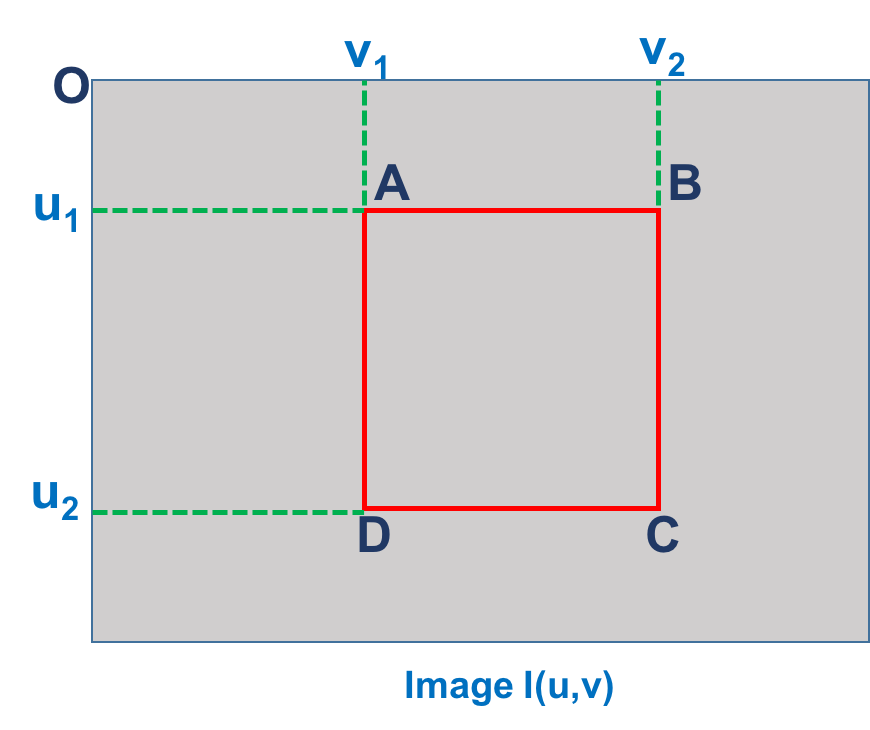
\includegraphics[scale=0.3]{integralimage.png}
	\end{figure}
	\begin{alertblock}{The Way to compute the filter's response}
		\begin{enumerate}
			\item Let $A, B, C, and D$ are the sum of all pixels in rectangle from $O$ to $A, B, C, and D$ respectively.
			\item The sum of pixels inside of rectangle $ABCD$ is $(C-B-D+A)$
		\end{enumerate}	
	\end{alertblock}
	
	
}
\frame{
	\frametitle{Convolution's implementation: Integral image}
	\selectlanguage{english}
	\textbf{CASE 2: 2D-array}
	\begin{figure}[!h]
		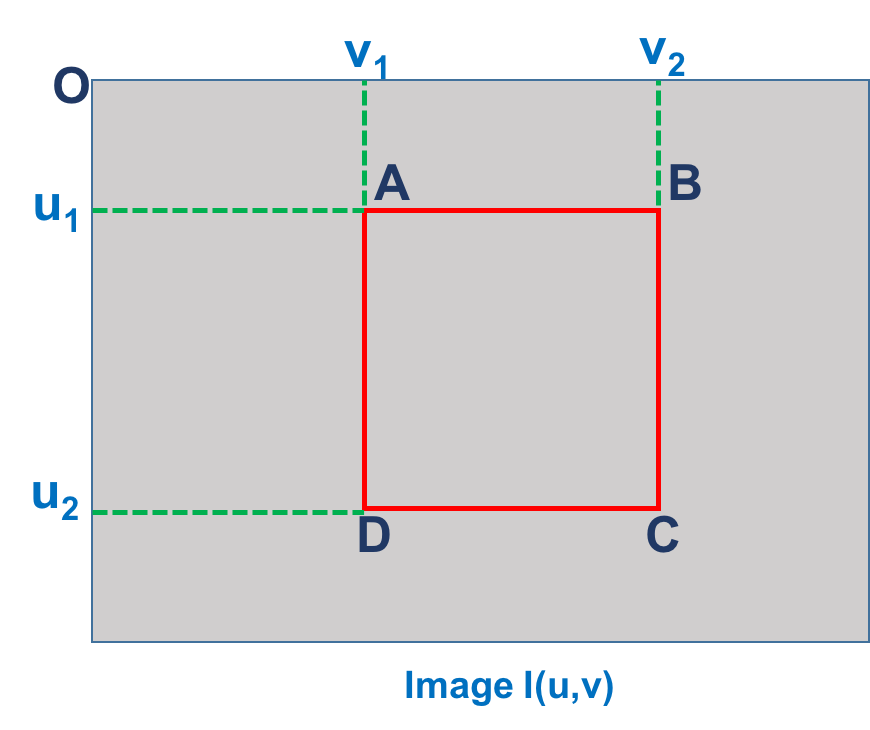
\includegraphics[scale=0.3]{integralimage.png}
	\end{figure}
	\begin{alertblock}{The Way to compute the filter's response}
		\begin{align}
			\nonumber
			I^{'}(u_2,v_2) 	&= C - B - D + A \\
			\nonumber
						&= S(u_2,v_2) - S(u_1,v_2) - S(u_2, v_1) + S(u_1, v_1)
		\end{align}
	\end{alertblock}
	
	
}

%%%%%%%%%%%%%%%%%%%%%%%%%%%%%%%%%%%%%%%%%%%%%%%

\end{document}